%These should be in an exercise environment. They should appear at the end of the chapter and the solutions at the end.
\section{Past Paper Problems}

\begin{exercise*} %N16HLP1-Q6
Consider the following recursive algorithm FUN(X, N), where X and N are two integers.	
	\begin{verbatim}
	FUN(X, N)
	if N<=0 then
	return 1
	else
	return X*FUN(X, N-1)
	end if
	\end{verbatim}
	The return statement gives the value that the algorithm generates.
	
	\begin{parts}
		\item Determine how many times multiplication is performed when this algorithm is executed.
		\begin{solution}
			N;
		\end{solution}
		\item Determine the value of FUN(2,3), showing all of your working.
		\begin{solution}
			Here's the solution.
			\begin{verbatim}
			FUN(2,3)=
			=2 * FUN(2,2) ;
			=2 * 2*FUN(2,1) ;
			=2 * 2 * 2 * FUN(2,0);
			=2*2*2*1= 8;
			\end{verbatim}
		\end{solution}
		\item State the purpose of this recursive algorithm.
		\begin{solution}
			Calculates $X^N$; Note: DO NOT accept vague answers that may suggest the understanding of $N^X$ or use incorrect terminology
		\end{solution}
	\end{parts}
\end{exercise*}



\begin{exercise*}%N16HLP1-Q9
A new higher level programming language is being developed.
\begin{parts}
\item Identify two reasons why consistent grammar and syntax should be essential features of a higher level programming language.
\begin{solution}
Easy to learn/use;
Otherwise time may be wasted learning the new language/writing programs in this HLL;
There will be no/less compilation errors;
There will be no/less logical errors;
(Reduction of time to create software;)
Future maintenance/development is possible by other programmers;
\end{solution}

\item Identify two features of a user interface that will allow application programmers to interact more easily with the programming language.
\begin{solution}
GUI;
Toolbars;
Menus;
Built in commands for inputting from touch screens;
Predicted text so that typing a class name followed by a full stop will bring up a list of methods/attributes;
Automatically use a colour to represent keywords/variables and improve readability
\end{solution}

\item State one method of providing user documentation.
\begin{solution}
Help files;
Online support;
\end{solution}
\end{parts}


Application programmers who use this programming language will be able to choose to use either an interpreter or a compiler.
\begin{parts}
\item Outline the need for an interpreter or a compiler.
	\begin{solution}
	Must be translated from a higher level language understandable by humans/not understood by machines;\\
	Must be translated into machine code;\\
	For the CPU to execute it;\\
	\end{solution}
\item Describe one advantage to application programmers of having both an interpreter and a compiler available.
	\begin{solution}
		Interpreter is faster/immediately warns about syntax errors/executes commands and they could use instead of the compiler while coding and debugging their programs;\\
		Compiler is required when there is a need to produce an executable version of a program;
	\end{solution}
\end{parts}
One of the predefined sub-programs in the new language is sumOdd(). It accepts an integer N as input. If $N <= 0$ it outputs -1, otherwise it outputs the sum of the first N odd numbers.
For example:\\
sumOdd(4) outputs 16, because 4 is not less than 0, and 1 + 3 + 5 + 7 = 16.
sumOdd(-3) outputs -1, because -3 is less than 0.
\begin{parts}
\item Construct, in pseudocode, the algorithm for sumOdd().
	\begin{solution}
		Example algorithm 1:
		\begin{verbatim}
		if N<=0 then
			S=-1
		else
			S=0
			loop for K=1 to N
				S=S+2*K-1
			endloop
		end if
		output S
		\end{verbatim}
Example algorithm 2:
	\begin{verbatim}
	if N>0 then	
		S=0	
		loop for K=1 to 2*N	
			if K mod 2==1 then	
				S=S+K	
			end if	
		endloop	
	else	
		S=-1	
	end if	
	output S
	\end{verbatim}

	\end{solution}
\item Outline the need for predefined sub-programs and collections.
\end{parts}
\end{exercise*}




\begin{exercise*}%N16HLP1-Q12
A two-dimensional array, A, has N rows and N columns, where N is a positive integer.
The following algorithm is written to fill array A with the numbers $1, 2, 3,\ldots N^2$.
\begin{verbatim}
N=input("Enter an integer greater than zero")
K=N*N
	loop for ROW=0 to N-1
		loop for COLUMN=0 to N-1
		A[ROW][COLUMN]=K
		K=K-1
		end loop
	end loop
\end{verbatim}

\begin{parts}
\item Trace the algorithm, with an input of $N=3$, to show the contents of array A after the algorithm has been executed.
	\begin{solution}
	This is the output of the array for each value:
	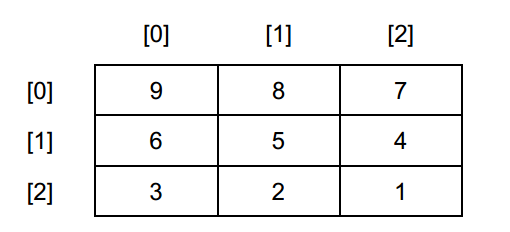
\includegraphics{topic_4_intro_programming/topic_4_exercises/arraySolution}
	\end{solution}
\end{parts}
There are many different ways of placing the numbers 1 to $N^2$ into an $N \times N$ two-dimensional array. 
The following two-dimensional array, with dimensions $5 \times 5$ has been filled in a circular (spiral) pattern with numbers 1 to $5^2$.

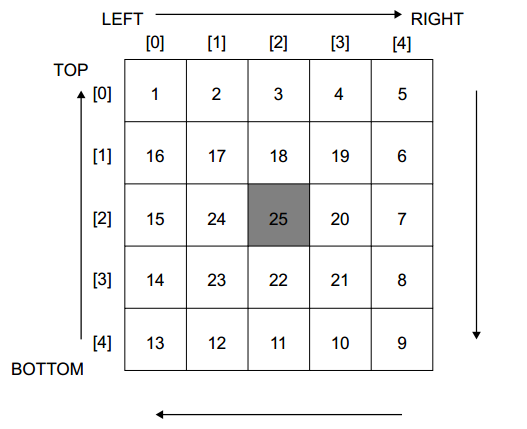
\includegraphics[scale=0.6]{topic_4_intro_programming/topic_4_exercises/array}
\newline

The general process of filling an $N \times N$ two-dimensional array, in a circular (spiral) pattern, with numbers from 1 to $N^2$ could be described as follows:

\begin{itemize}
\item initialize Z=1,
\item initialize TOP, BOTTOM, LEFT and RIGHT,
\item iterate until the whole array is filled,
\item each time Z is placed correctly increase the value of Z by 1,
\item fill the elements of the TOP row starting from LEFT to RIGHT,
\item increase TOP by 1 before filling the elements of the RIGHT column,
\item fill the elements of the RIGHT column starting from TOP to BOTTOM,
\item decrease RIGHT by 1 before filling the elements of the BOTTOM row,
\item and continue filling the BOTTOM row and LEFT column in a similar way, adjusting TOP, RIGHT, BOTTOM and LEFT accordingly.
\end{itemize}

\begin{parts}
\item State the initial values for TOP, BOTTOM, LEFT and RIGHT.
	\begin{solution}
	TOP=0
	BOTTOM=N-1
	LEFT=0
	RIGHT=N-1
	\end{solution}
\item State the consequence of not increasing TOP by 1 before starting to fill the elements of the RIGHT column.
	\begin{solution}
	\newline
	The array element at position [TOP][RIGHT] in which value of Z is already placed, will be overwritten by the value of Z + 1;\\
	Not all of the numbers 1 to $N^2$ will be placed in the array because some will be overwritten;\\
	The array will be filled with more than $N^2$ numbers/with numbers greater than $N^2$;\\
	Accept answers from the sample $5 \times 5$ table, eg the value of MATRIX[0][4] which is already filled by 5, will be changed to 6.
	\end{solution}
\item In the algorithm described above, state the indices (subscripts) of the first and the last element to be filled in the BOTTOM row.
	\begin{solution}
	The first element to be filled in BOTTOM row has indices (subscripts) [BOTTOM][RIGHT] and the last to be filled has indices (subscripts) [BOTTOM][LEFT];
	\end{solution}
\item Construct, in pseudocode, an algorithm to fill an $N \times N$ two-dimensional array, in a circular (spiral) pattern, with numbers from 1 to $N^2$ as described above.

\end{parts}
\end{exercise*}